\documentclass[journal]{IEEEtran}

\usepackage{cite}
\usepackage{url}
\usepackage{graphicx}
\usepackage{minted}

\setminted{
    fontsize=\small,
    breaklines,
    bgcolor=gray!5
}

\begin{document}

\title{VIP: A Modal Terminal-Based Text Editor in C}
\author{Alexandros~Papagrigoriou,~Alexios~Lagios~it2023092}

\maketitle

\begin{center}
    
\includegraphics[width=0.15\textwidth]{images/vip-logo.png}
\end{center}

\begin{abstract}
The development of text editors provides valuable insight into systems programming, software architecture, and user interface design. Modal text editors such as Vim remain a cornerstone of efficient, keyboard-driven text editing, yet their internal architecture is rarely examined in depth in academic settings. This paper presents VIP ("Vi rIPoff"), a from-scratch implementation in C of a modal, terminal-based text editor that reproduces a subset of Vim's normal, insert, visual, and command modes. The system is built directly on POSIX terminal primitives, without external editing or rendering libraries, and implements a dynamic buffer, a stateful command parser supporting operator-motion composition, a rich set of cursor motions including word, paragraph, and bracket-matching navigation, and a minimal command line supporting file I/O and editor options. We describe the system's architecture, the design decisions behind its data structures and input-parsing model, and discuss the engineering trade-offs encountered when reimplementing a portion of Vim's modal grammar. We conclude with an evaluation of functional coverage against real Vim, a discussion of current limitations such as the absence of an undo system and a yank/paste register, and directions for future work.
\end{abstract}

\section{Introduction}
\IEEEPARstart{T}{ext} editors are among the most frequently used pieces of software in a programmer's daily workflow, and modal editors -- most notably Vim and its predecessor vi -- have endured for decades because of the efficiency offered by their command grammar. In a modal editor, the same physical keys perform different actions depending on the current editing mode (e.g. "normal" mode for navigation and manipulation versus "insert" mode for typing text), and commands are frequently composed of an operator and a motion (for example, d for delete combined with w for word produces dw, "delete to the next word").

This project, named VIP, is a terminal-based text editor written in C that reimplements a subset of this Vim-based modal grammar. The motivation for the project was twofold. First, it serves as a practical exercise in systems programming: the editor interacts directly with the terminal through POSIX APIs, manages dynamic memory for an arbitrarily large text buffer, and must remain responsive under raw keyboard input. Second, it serves as a study of language design in miniature -- Vim's command grammar can be viewed as a small formal language, and parsing it correctly (including handling numeric counts, operator-pending states, and multi-key motions) is a non-trivial state-machine design problem.

The remainder of this paper is organized as follows. Section 2 describes the overall architecture of the system and the responsibilities of each module. Section 3 discusses the core data structures used to represent text. Section 4 details the design of the input-handling and command-parsing subsystem, including how the operator-motion composition is implemented. Section 5 describes the rendering and terminal-interaction layer. Section 6 evaluates the editor against the goals of the project and against real Vim in terms of feature coverage. Section 7 discusses limitations and future work, and Section 8 concludes.

\section{System Architecture}
VIP is organized as a set of cooperating C modules, each with a single, clearly scoped responsibility. The project is built with a Makefile, producing separate debug and release binaries, and is compiled with strict warning flags (-Wall -Wextra -Wpedantic -Werror) to enforce code quality.

The high-level module breakdown is as follows. The architecture of VIP is illustrated in Fig.~\ref{fig:system-architecture}.

\begin{figure}[htbp]
    \centering
    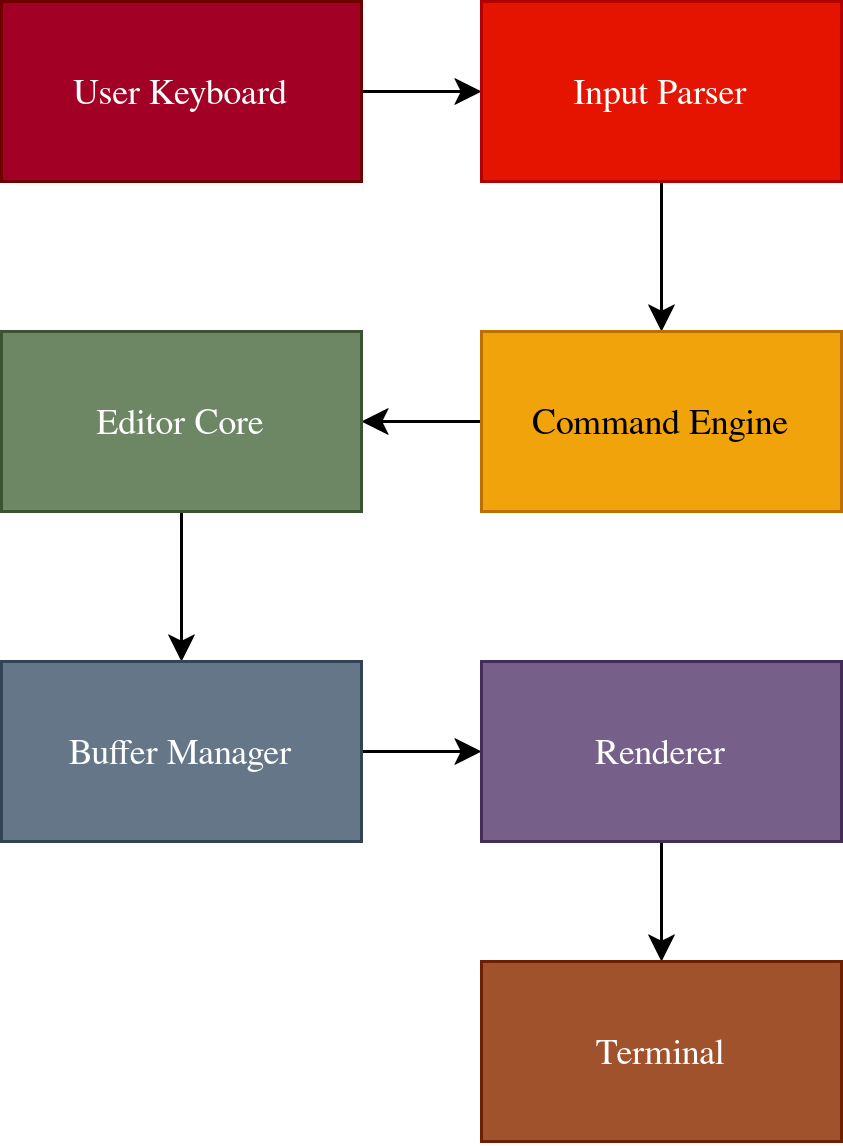
\includegraphics[width=\columnwidth]{images/system-architecture.png}
    \caption{High-level system architecture of VIP.}
    \label{fig:system-architecture}
\end{figure}

\begin{itemize}
    \item terminal -- raw-mode terminal control and window-size detection.
    \item line and buffer -- the core text-storage data structures, described in detail in Section~\ref{sec:data-structures}.
    \item editor -- the central Editor struct, which contains the text buffer, cursor state, current mode, and command-line state into a single context object.
    \item parser -- a small state machine (Parser) that interprets sequences of key presses as editor commands, dispatching to mode-specific handlers.
    \item normal, insert, visual, command -- one handler module per editor mode, each implementing the key-handling logic specific to that mode.
    \item motion and movement -- implementations of Vim-style cursor motions (word, line, paragraph, bracket-matching, character search, etc.) and the logic that distinguishes pure cursor movement from operator-bound motions.
    \item draw -- the rendering subsystem responsible for redrawing the visible buffer, status line, and command line using ANSI escape sequences.
    \item fileio -- loading files into the buffer and writing the buffer back to disk.
    \item error and colors -- centralized error handling (with cleanup of terminal state on fatal errors) and ANSI color/formatting constants.
\end{itemize}

At runtime, the program enters an alternate terminal screen, switches the terminal into raw mode (disabling line buffering, echo, and signal generation for keys such as Ctrl-C), and enters a main loop. Each iteration of the loop reads a single key, dispatches it to the parser, recomputes the visible scroll position based on the cursor, updates the status line, and redraws the screen. On exit -- triggered by the :q, :wq, or :x command-line commands -- the loop terminates, the terminal is restored to its original mode, and the alternate screen is exited, returning the user's shell to its prior state.

\section{Data Structures}
\label{sec:data-structures}

\subsection{The Line structure}
Each line of text is represented by a Line struct containing a character array, a length field, and a capacity field. The line\_ensure function grows the backing array by 1.5x whenever an insertion would exceed the current capacity, avoiding the cost of repeated single-character insertions to O(1) on average. A companion function, line\_compact, shrinks the array back down when a line becomes much shorter than its allocated capacity (for example, after a large deletion), preventing memory from being permanently wasted on lines that were once long but have since been trimmed.

\begin{minted}{C}
// line.h

#include <stddef.h>

typedef struct {
    char* chars;
    size_t length;
    size_t capacity;
} Line;
\end{minted}

\subsection{The Buffer structure}
The Buffer struct is a dynamic array of Line structs, with its own capacity and line\_count fields and the same grow/compact strategy. This gives the whole-file representation the same performance characteristics as the per-line representation: appending a new line (as happens when the user presses Enter in insert mode, or o/O in normal mode) is an O(1) operation, while operations that touch the middle of the buffer -- such as inserting or deleting a line -- require an O(n) memmove of the trailing lines, where n is the number of lines after the affected position.

All buffer-mutating operations (insert\_char, insert\_string, insert\_enter, insert\_backspace, etc.) take a pointer to the cursor Position and update it in place, so that cursor position is updated based on the action to the buffer. This was a deliberate design choice to avoid an entire class of bugs in which the cursor points to old memory after a buffer action.

\begin{minted}{C}
// buffer.h

#include <stddef.h>

#include "line.h"

typedef struct {
    Line* lines;
    size_t line_count;
    size_t capacity;
} Buffer;
\end{minted}


\subsection{The Editor context}
The Editor struct is the central piece of mutable state for the whole program. It holds the Buffer itself; the cursor Position (in buffer coordinates); a text Position representing the top-left corner of the visible viewport (used for scrolling); the current Mode (an enum with values NORMAL, INSERT, VISUAL, VISUAL\_LINE, COMMAND, and EXIT); a CommandLine struct holding the contents and cursor position of the command line; and several small flags such as number and relative\_number (corresponding to Vim's :set number and :set relativenumber options) and saved (tracking whether the buffer has unsaved changes, used to implement Vim's familiar "No write since last change" guard on :q).

\begin{minted}{C}
// editor.h

#include <stdbool.h>
#include <stddef.h>

#include "buffer.h"

typedef enum {
    NORMAL,
    INSERT,
    VISUAL,
    VISUAL_LINE,
    COMMAND,
    EXIT
} Mode;
\end{minted}

\begin{minted}{C}
typedef struct {
    char line[COMMAND_LINE_SIZE];
    size_t cursor_col;
    size_t length;
} CommandLine;
\end{minted}

\begin{minted}{C}
typedef struct {
    Buffer buffer;
    Position cursor;
    bool successful_motion;
    bool save_curosr_col;
    size_t prev_cursor_col;
    Position text;
    bool number;
    bool relative_number;
    char key_cache_string[...];
    char cursor_position_string[...];
    CommandLine command_line;
    bool saved;
    bool in_start;
    Mode mode;
    char* filename;
} Editor;
\end{minted}

\section{Input Handling and Command Parsing}
The most interesting part of the project is the command-parsing subsystem, because Vim's normal-mode grammar is not a flat list of single-key commands but a small language. A command may consist of an optional numeric count, an optional operator (such as d for delete, c for change, or y for yank), an optional second numeric count (applied after the operator), and a motion that the operator acts upon. For example, 2d3w means "delete three words two times" (the two counts multiply), and c\$ (same as C) means "change the contents until the end of the line".

\subsection{The Parser state machine}
VIP models this grammar with a small Parser struct containing a state field (NORMAL or OPERATOR\_PENDING) and a cmd field containing the count on how many times to execute the command, the operator, the motion, and an argument if needed. Each key press is fed to the parser, which incrementally builds up this cmd structure. Digits are added to the execution count; letters such as d, c, and y transition the parser into STATE\_OPERATOR\_PENDING; and motion keys (h, j, k, l, w, b, e, and so on) set the motion field and, if the command is now complete, the command gets executed by calling the appropriate handler and then resets the parser to its initial state.

\begin{minted}{C}
// parser.h

#include <stddef.h>

#include "motion.h"
#include "operator.h"

typedef struct {
    char chars[...];
    int length;
} KeyCache;

\end{minted}

\begin{minted}{C}
typedef struct {
    size_t count;
    size_t count_after_operator;
    Operator operator;
    Motion motion;
    char argument;
    KeyCache key_cache;
} Command;
\end{minted}

\begin{minted}{C}
typedef enum {
    STATE_NORMAL,
    STATE_OPERATOR_PENDING
} ParserState;
\end{minted}

\begin{minted}{C}
typedef struct {
    ParserState state;
    Command cmd;
} Parser;
\end{minted}

The Parser state machine of VIP is illustrated in Fig.~\ref{fig:parser-state-machine}.

\begin{figure}[htbp]
    \centering
    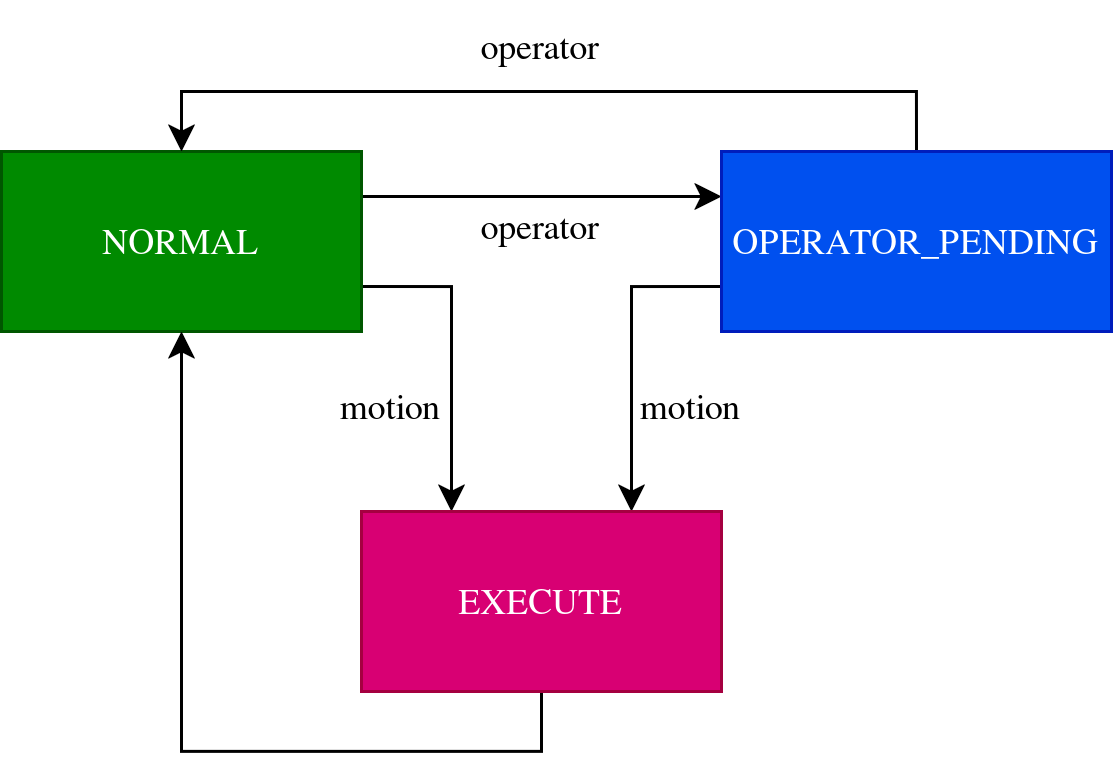
\includegraphics[width=\columnwidth]{images/parser-state-machine.png}
    \caption{Parser state machine of VIP.}
    \label{fig:parser-state-machine}
\end{figure}

\subsection{Operators and execution}
Once a complete command has been assembled, \texttt{execute normal mode} dispatches on the motion's type.

The MotionType enum has five values --- \texttt{NONE}, \texttt{ROW}, \texttt{COL\_LEFT}, \texttt{COL\_RIGHT}, and \texttt{POSITION}. However, \texttt{NONE} is never produced by valid input, and both column types behave identically in execution.

In practice, the system only handles three motion shapes: row, column, and position.

This reduction is what makes the operator-motion combinations tractable. Rather than writing a separate implementation for every (operator, motion) pair -- which for d, c, y, and the twenty-plus motions in motion.c would mean dozens of cases -- each motion module is responsible only for answering a single question: "given the current cursor position and this motion, where does the cursor end up?". \texttt{get\_motion} functions compute exactly this target and report it back via the editor's \texttt{successful\_motion} flag (which is cleared if the motion is not applicable, e.g. j on the last line). The executor then performs the motion itself by moving the cursor to that target, completely independently of which operator, if any, is active.

Only once the target has been computed does the operator come into play. The operator itself, \texttt{OP\_DELETE}, \texttt{OP\_CHANGE}, or \texttt{OP\_YANK}, is then just a three-way switch on "what to do with this range", applied identically regardless of which motion produced the range. The net effect is that adding a new motion only requires implementing its target-computation function; it is automatically compatible with every existing operator, and conversely a new operator only needs to handle three range shapes rather than one per motion.

\begin{minted}{C}
// motion.h

typedef enum {
    MOT_TYPE_NONE,
    MOT_TYPE_ROW,
    MOT_TYPE_COL_LEFT,
    MOT_TYPE_COL_RIGHT,
    MOT_TYPE_POSITION
} MotionType;
\end{minted}

\begin{minted}{C}
// normal.c

static void execute_row_motion(Parser* parser, Editor* editor) {
    size_t row = get_motion_row(editor, parser->cmd.motion, parser->cmd.count);

    if (!editor->successful_motion) {
        editor->save_curosr_col = false;
        return;
    }

    if (parser->cmd.operator == OP_NONE) {
        editor->cursor.row = row;
        return;
    }

    switch (parser->cmd.operator) {
        case OP_DELETE:
            ...
        case OP_CHANGE:
            ...
        case OP_YANK:
            ...
        default:
            ERROR("Wrong operator");
    }
}
\end{minted}

\begin{minted}{C}
static void execute_col_motion(Parser* parser, Editor* editor) {
    size_t col = get_motion_col(editor, parser->cmd.motion, parser->cmd.count, parser->cmd.argument);

    if (!editor->successful_motion) {
        editor->save_curosr_col = false;
        return;
    }

    if (parser->cmd.operator == OP_NONE) {
        editor->cursor.col = col;
        return;
    }

    switch (parser->cmd.operator) {
        case OP_DELETE:
            ...
        case OP_CHANGE:
            ...
        case OP_YANK:
            ...
        default:
            ERROR("Wrong operator");
    }
}
\end{minted}

\subsection{Modes beyond normal mode}
Insert mode (\texttt{insert.c}) is comparatively simple: printable characters are inserted at the cursor via \texttt{insert\_string} and other special keys like \texttt{Enter} and \texttt{Backspace} call specific \texttt{buffer} functions to modify text. Visual mode (\texttt{visual.c}, \texttt{visual\_line.c}) reuses the same motion infrastructure as normal mode to extend a selection anchored at the position where v or V was pressed, although at the time of writing the operators that act on a visual selection (d, c, y) are not yet fully wired up -- this is discussed in further detail in Section~\ref{sec:limitations-and-future-work}.

Command mode (\texttt{command.c}) implements a minimal command line. After stripping leading/trailing whitespace, the input is classified as either a bare line number (triggering a jump to that line)  or as one of a small set of recognized commands: \texttt{:w} / \texttt{:write}, \texttt{:q} / \texttt{:quit}, etc. and \texttt{:set} followed by an option name. Unrecognized commands produce "Not an editor command: \{name\}" message in the status line, and attempting \texttt{:q} / \texttt{:quit} with unsaved changes produces "No write since last change" error.

The mode transition in VIP is illustrated in Fig.~\ref{fig:mode-transition}.

\begin{figure}[htbp]
    \centering
    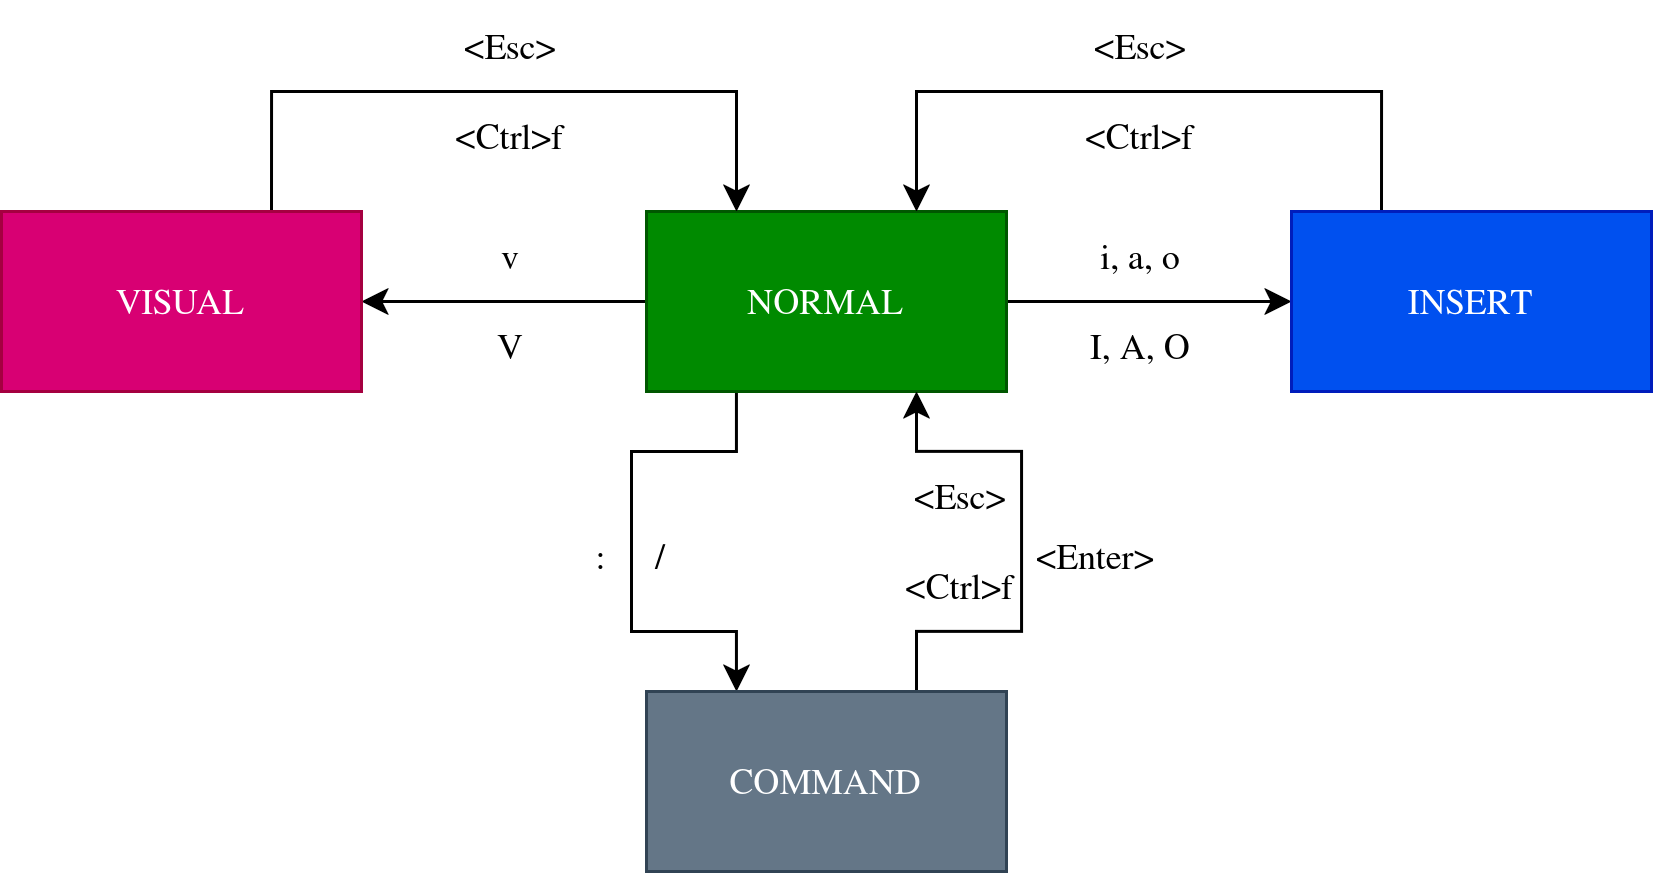
\includegraphics[width=\columnwidth]{images/mode-transition.png}
    \caption{Mode transition in VIP.}
    \label{fig:mode-transition}
\end{figure}

\begin{minted}{C}
// normal.c

switch (key) {
    case 'i':
        editor->mode = INSERT;
        parser_init(parser);
        return;
    case 'a':
        editor->mode = INSERT;
        insert_arrow_right(editor);
        parser_init(parser);
        return;
    case 'I':
        editor->mode = INSERT;
        editor->cursor.col = get_motion_col(editor, MOT_FIRST_NON_BLANK_CHAR_OF_LINE);
        parser_init(parser);
        return;
    case 'A':
        editor->mode = INSERT;
        editor->cursor.col = get_motion_col(editor, MOT_END_OF_LINE);
        insert_arrow_right(editor);
        parser_init(parser);
        return;
    case 'o':
        editor->mode = INSERT;
        append_line(&editor->buffer, &editor->cursor);
        parser_init(parser);
        return;
    case 'O':
        editor->mode = INSERT;
        prepend_line(&editor->buffer, &editor->cursor);
        parser_init(parser);
        return;
    case 'v':
        editor->mode = VISUAL;
        parser_init(parser);
        return;
    case 'V':
        editor->mode = VISUAL_LINE;
        parser_init(parser);
        return;
    case ':':
    case '/':
        editor->mode = COMMAND;
        parser_init(parser);
        return;
}
\end{minted}

\begin{minted}{C}
// other modes

switch (key) {
    case ESC:
    case CTRL_F:
        editor->mode = NORMAL;
        editor->command_line.line[0] = '\0';
        break;
    case ...:
        ...;
}
\end{minted}

\section{Terminal Interaction and Rendering}
VIP performs all input and output through raw POSIX terminal calls. On startup, \texttt{enable raw mode} uses tcgetattr/tcsetattr to disable canonical mode, echo, and signal generating control characters, while \texttt{enter alt screen} switches to the terminal's alternate screen buffer. The terminal's dimensions are queried via the \texttt{TIOCGWINSZ ioctl}, and a \texttt{SIGWINCH} handler triggers a redraw whenever the terminal is resized.

\begin{minted}{C}
// vip.c

void cleanup(void) {
    free_editor(&editor);

    disable_raw_mode();
    exit_alt_screen();
}

void run_vip(char* filename) {
    enter_alt_screen();
    enable_raw_mode();

    editor_init(&editor, filename);

    signal(SIGWINCH, handle_resize);
    update_window_size();

    while (editor.mode != EXIT) {
        // main loop
    }

    cleanup();
}
\end{minted}

\begin{minted}{C}
// terminal.c

void enable_raw_mode(void) {
    tcgetattr(STDIN_FILENO, &original);

    struct termios raw = original;
    raw.c_lflag &= ~(ECHO | ICANON | ISIG);
    raw.c_iflag &= ~(IXON | ICRNL);
    tcsetattr(STDIN_FILENO, TCSAFLUSH, &raw);
}

void disable_raw_mode(void) {
    tcsetattr(STDIN_FILENO, TCSAFLUSH, &original);
}

void update_window_size(void) {
    struct winsize w;
    ioctl(STDOUT_FILENO, TIOCGWINSZ, &w);
    max_screen.row = w.ws_row;
    max_screen.col = w.ws_col;

    draw_window();

    refresh_window();
}
\end{minted}

Each iteration of the main loop performs a full redraw: the screen is cleared, the cursor is hidden (to avoid visible flicker while redrawing), the visible portion of the buffer is printed line-by-line with optional line numbers, a status line is drawn showing the current mode, the accumulated key sequence (useful for understanding pending multi-key commands), and the cursor's row/column position, and finally the cursor is repositioned and shown again. The viewport-scrolling logic implements "scrolloff" behavior, keeping the cursor at least eight lines away from the top or bottom edge of the visible area where possible.

\section{Evaluation}

\subsection{Motion references}
Below there are the motions implemented in \texttt{motion.c}, the key (or key sequence) that triggers each one, and the resulting cursor behavior. These motions form the navigation vocabulary of the editor and are modeled after the corresponding motions in Vim. In addition to simple character and line-based movement, VIP supports word navigation, paragraph navigation, bracket matching, and character-search motions. The motion subsystem is designed so that each motion computes a target location relative to the current cursor position. This target can be used either for ordinary cursor movement or as the range operand of an editing operator such as delete or change. As a result, the same motion implementation can be reused across a large number of operator-motion combinations without duplicating logic.

\begin{table}[htbp]
\centering
\caption{Supported motions in VIP}
\label{tab:motions}
\begin{tabular}{ll}
\hline
Key & Description \\
\hline
\texttt{h} / Left & move cursor left \\
\texttt{j} / Down & move cursor down \\
\texttt{k} / Up & move cursor up \\
\texttt{l} / Right & move cursor right \\
\texttt{w} & jump forwards to the start of a word \\
\texttt{W} & jump forwards to the start of a big word \\
\texttt{e} & jump forwards to the end of a word \\
\texttt{E} & jump forwards to the end of a big word \\
\texttt{b} & jump backwards to the start of a word \\
\texttt{B} & jump backwards to the start of a big word \\
\texttt{\%} & move cursor to matching character \\
\texttt{0} & jump to the start of the line \\
\texttt{\^} & jump to the first non-blank character of the line \\
\texttt{\$} & jump to the end of the line \\
\texttt{gg} &  go to the first line of the document \\
\texttt{G} & go to the last line of the document \\
\texttt{f\{c\}} & jump to next occurrence of character \{c\} \\
\texttt{t\{c\}} & jump to before next occurrence of character \{c\} \\
\texttt{F\{c\}} & jump to the previous occurrence of character \{c\} \\
\texttt{T\{c\}} & jump to after previous occurrence of character \{c\} \\
\texttt{\}} & jump to next paragraph \\
\texttt{\{} & jump to previous paragraph \\
\hline
\end{tabular}
\end{table}

The semantics of each motion were verified against the official Vim documentation \cite{vimhelp}, to ensure that VIP's behavior matches that of real Vim for the implemented subset.

\subsection{Code quality and build process}
The project is compiled with -Wall -Wextra -Wpedantic -Werror, meaning that any compiler warning is treated as a build failure. This was chosen to enforce a high standard of memory and type safety given that the project is written in C and performs extensive manual memory management (malloc/realloc/free) across the Line and Buffer structures. A separate debug build (with -g3 -O0 -DDEBUG) enables source-location-annotated error messages and is suitable for use with gdb, while the release build (-O2 -flto, stripped) is optimized for normal use. The codebase is organized with a strict separation between interface (\texttt{include/}) and implementation (\texttt{src/}), with each module exposing a minimal public API through its header.

\subsection{Error handling}
Centralized error handling, implemented in \texttt{error.c} via the ERROR macro, ensures that any fatal internal error (such as a memory-allocation failure or an out-of-bounds row/column access) first calls \texttt{cleanup()} -- which restores the terminal to the original mode and exits the alternate screen -- before printing a diagnostic and terminating. This prevents the common failure mode of full-screen terminal applications leaving the user's shell in raw mode or on the alternate screen after a crash, which would otherwise require the user to blindly type reset to recover.

\begin{minted}{C}
// error.h

#ifdef NDEBUG
#define ERROR(msg) error(msg, NULL, 0, NULL)
#else
#define ERROR(msg) error(msg, __FILE__, __LINE__, __func__)
#endif

void error(const char* msg, const char* file, int line, const char* func);
\end{minted}

\begin{minted}{C}
// error.c

void error(const char* msg, const char* file, int line, const char* func) {
    cleanup();

#ifdef NDEBUG
    (void)file;
    (void)line;
    (void)func;
    fprintf(stderr, "Error: %s\n", msg);
#else
    fprintf(stderr, "Error: %s (%s:%d, %s)\n", msg, file, line, func);
#endif

    fflush(stderr);

    exit(EXIT_FAILURE);
}
\end{minted}

\section{Limitations and Future Work}
\label{sec:limitations-and-future-work}
Several areas of the project are explicitly marked as incomplete or were out of scope for the current iteration:

\begin{enumerate}
    \item Undo/redo. Vim's undo tree is one of its most heavily used features, and VIP currently has no undo mechanism at all.
    \item Yank, delete, and paste registers. The y operator and the p/P paste commands are not yet implemented; the parser recognizes y as an operator but the corresponding function is not yet implemented.
    \item Visual mode operators. Visual mode currently allow extending a selection but do not yet apply d, c, or y to that selection.
    \item Search. The / command-line prefix is recognized and routed to execute\_search, but the function is empty; implementing it would require a substring-matching pass over the buffer.
\end{enumerate}

\section{Conclusion}
VIP demonstrates that a meaningful and usable subset of Vim's modal editing model can be implemented in a moderate amount of well-organized C code, using only POSIX terminal facilities and standard dynamic-memory techniques. The project's most significant contribution, from an academic perspective, is its explicit and reasonably clean state-machine formulation of Vim's operator-motion grammar -- the separation between motion computation, and operator execution provides a template that could be extended to cover the remaining parts of Vim's command language (undo and search) without a fundamental redesign. While several features remain unimplemented, the existing codebase -- spanning terminal handling, a dynamic text buffer, a composable command parser, and a redraw-based renderer -- already constitutes a working terminal editor capable of opening, navigating, editing, and saving real text files using familiar Vim keybindings.

\bibliographystyle{IEEEtran}
\bibliography{bibtex/bib/references}

\end{document}
